\chapter{Engineering Implementation and Prediction Mechanisms of NFF}
\label{chap:implementation}

\section{Code Optimization Strategies}
\label{sec:optimization_strategies}

To reduce the execution time per filtering step, this study implements four optimization strategies in the Julia environment\cite{JULIA}.

\subsection{Zero-Allocation and Type Stability}
\label{subsec:zero_allocation}

\paragraph{Implementation of zero allocation} In high-level programming languages, dynamic memory allocation and garbage collection (GC) are major sources of computational overhead. The iterative computations of NFF involve a large number of intermediate and output variables. To avoid this overhead, a zero-allocation strategy is adopted during initialization: fixed-size contiguous memory is preallocated for all intermediate variables, including the gradient vector $\mJ$ and the Hessian matrix $\mH$. During the subsequent filtering loops, all mathematical operations are performed in place, with results written directly into the preallocated memory locations. This strategy eliminates repeated memory allocation and deallocation during execution and substantially improves computational efficiency.

\paragraph{Comparison of Dynamic and Zero Allocation in Julia}
To illustrate the practical impact of this strategy, the following conceptual Julia implementation is provided. The first nested loop simulates naive dynamic allocation, while the second demonstrates the proposed zero-allocation approach using preallocated memory buffers (\texttt{J\_prealloc} and \texttt{H\_prealloc}).
\clearpage
\begin{lstlisting}[
    caption={Julia implementation of zero-allocation strategy.},
    label={lst:zero_allocation_julia},
    basicstyle=\small\ttfamily,
    frame=single,
    breaklines=true]
using BenchmarkTools

function filter_loop_allocating(iterations, dim)
    total_loss = 0.0
    for i in 1:iterations
        # Dynamic allocation: Memory requested in each iteration
        J = zeros(Float64, dim)
        H = zeros(Float64, dim, dim)

        for j in 1:dim
            J[j] = i * 0.1
            H[j, j] = i * 0.2
        end
        total_loss += sum(J) + sum(H)
    end
    return total_loss
end

function filter_loop_zero_alloc!(
    iterations, dim, J_prealloc, H_prealloc)
    total_loss = 0.0
    for i in 1:iterations
        # Zero allocation: Overwriting preallocated memory directly
        fill!(J_prealloc, 0.0)
        fill!(H_prealloc, 0.0)

        for j in 1:dim
            J_prealloc[j] = i * 0.1
            H_prealloc[j, j] = i * 0.2
        end
        total_loss += sum(J_prealloc) + sum(H_prealloc)
    end
    return total_loss
end
\end{lstlisting}
\begin{Remark}[Verification of Zero Allocation]
The \texttt{@btime} macro from the \texttt{BenchmarkTools} package evaluates execution time and exact memory allocations. An output of \texttt{0 allocations} confirms that no garbage collection overhead is introduced.
\end{Remark}

\paragraph{Strict type stability} If variable types are not known at compile time, the program must perform dynamic dispatch during runtime for each arithmetic operation. To eliminate this overhead, this study strictly enforces type consistency for all data structures during memory allocation and function definition. In particular, the Hessian matrix $\mH$, the gradient vector $\mJ$, and all related intermediate variables are explicitly declared as \texttt{Float64}.

\paragraph{Comparison of Type-Unstable and Type-Stable Implementations}
To illustrate the practical impact of strict type stability, the following conceptual Julia implementation is provided. The first function simulates a type-unstable accumulator where the variable type changes dynamically during execution. The second demonstrates the proposed type-stable approach by explicitly matching the initialization type with the input array's element type, completely avoiding dynamic dispatch.
\clearpage
\begin{lstlisting}[
    caption={Julia implementation demonstrating type stability.},
    label={lst:type_stability_julia},
    basicstyle=\small\ttfamily,
    frame=single,
    breaklines=true]
# 1. Type-Unstable Implementation (Dynamic Dispatch)
function unstable_sum(arr)
    s = 0  # Initialized as Int64
    for x in arr
        # Type changes to Float64 if arr contains floats
        s = s + x  
    end
    return s
end

# 2. Type-Stable Implementation (Zero Dynamic Dispatch)
function stable_sum(arr)
    s = 0.0  # Explicitly initialized as Float64
    for x in arr
        # Type remains concrete (Float64) throughout the loop
        s = s + x  
    end
    return s
end
\end{lstlisting}

\begin{Remark}[Verification of Type Stability]
The \texttt{@code\_warntype} macro evaluates the type inference. In practice, type instability can be diagnosed directly by observing the output colors in the terminal: variables inferred as non-concrete types (such as \texttt{Any} or \texttt{Union}) are highlighted in \textbf{red} or \textbf{yellow}, immediately confirming the presence of runtime dynamic dispatch.
\end{Remark}

\paragraph{Bounds-check elimination} To ensure memory safety, Julia performs bounds checking by default during every array and matrix access. In NFF, constructing the Hessian matrix $\mH$ and the gradient vector $\mJ$ requires $L \times L$ nested loops, and repeated bounds checking becomes very costly. Since the particle number $L$ is deterministic and all arrays are strictly initialized during the zero-allocation phase, the mathematical structure of the algorithm guarantees that no out-of-bounds access occurs. Therefore, this study applies the \texttt{@inbounds} macro to each loop, instructing the compiler to skip array bounds checking.

\subsection{Utilizing Symmetry and Avoiding Redundant Calculations}
\label{subsec:avoiding_redundant}

In the NFF algorithm, the most computationally expensive task is the evaluation of the gradient $\mJ$ and the Hessian $\mH$. According to the theoretical derivation, both quantities depend on pairwise interactions among all particles. A naive implementation therefore has a time complexity of $\mathcal{O}(L^2)$.

For CPU-based computation, the main optimization objective is to minimize the total number of floating-point operations. Since computing $\mJ$ and $\mH$ requires iterating over all particle pairs, the process can be represented by a two-dimensional table of pairwise differences $\vd$:

\begin{Table}[ht]
	\begin{tabular}{c|ccccc}
		\hline
		Pairwise differences $\vd$ & $\vx_1$ & $\vx_2$ & $\vx_3$ & $\cdots$ & $\vx_L$ \\ \hline
		$\vx_1$ & \vzero & $\vx_1 - \vx_2$ & $\vx_1 - \vx_3$ & $\cdots$ & $\vx_1 - \vx_L$ \\
		$\vx_2$ & $\vx_2 - \vx_1$ & \vzero & $\vx_2 - \vx_3$ & $\cdots$ & $\vx_2 - \vx_L$ \\
		$\vx_3$ & $\vx_3 - \vx_1$ & $\vx_3 - \vx_2$ & \vzero & $\cdots$ & $\vx_3 - \vx_L$ \\
		$\vdots$ & $\vdots$ & $\vdots$ & $\vdots$ & $\ddots$ & $\vdots$ \\
		$\vx_L$ & $\vx_L - \vx_1$ & $\vx_L - \vx_2$ & $\vx_L - \vx_3$ & $\cdots$ & \vzero \\ \hline
	\end{tabular}
	\caption{Pairwise particle differences.}
	\label{tab:particle_diff}
\end{Table}

The following observations can be made from \Tab{tab:particle_diff}:

When $\vd = \vzero$, the gradient term satisfies $\mathcal{G}(\vzero) = \vzero$, and the Hessian term is given by $\mathcal{H}(\vzero) = \log(d_\text{min}^2)\mI$. Since these diagonal terms are constants, they can be assigned directly outside the main loop, allowing the iteration to skip the diagonal entries.

The upper and lower triangular parts of the table are symmetric (e.g., $\vx_2 - \vx_1 = -(\vx_1 - \vx_2)$). Because the algorithm depends heavily on the squared Euclidean distance $\vd^{\top}\vd$, the sign of the difference does not affect the scalar result. As a result, the number of required evaluations is reduced from $L^2$ to $\frac{L(L-1)}{2}$ by computing only the lower triangular part. The remaining $\frac{L(L+1)}{2}$ operations are reduced to simple memory writes or accumulation operations.

Furthermore, the gradient $\mathcal{G}(\vd)$ and the Hessian $\mathcal{H}(\vd)$ have very similar mathematical structures. Both involve expensive operations such as $\vd^{\top}\vd$, $\frac{1}{d_{\text{min}}^2 + \vd^{\top}\vd}$, and $\log(d_\text{min}^2 + \vd^{\top}\vd)$. To achieve a significant speedup, all intermediate quantities for both $\mJ$ and $\mH$ are therefore computed simultaneously in a single pass over each particle pair $(\vx_k, \vx_l)$, instead of being evaluated separately.

In addition, Julia uses a column-major memory layout. This means that consecutive elements in the same column of a matrix are contiguous in memory, whereas elements in the same row are not.

To avoid performance degradation caused by cache misses, the block matrix $\mH$ must therefore be filled column by column. Moreover, since $\mH$ is symmetric, the algorithm computes and stores only the lower triangular part, thereby further reducing the number of costly memory writes. Finally, by using Julia's \texttt{Symmetric} wrapper, the computational cost of subsequent operations involving $\mH$ is effectively halved.

\begin{algorithm}[ht]
	\caption{Calculation of Gradient $\mJ$ and Hessian $\mH$}
	\label{alg:calc_JH}
	\begin{algorithmic}[1]
		\STATE \textbf{Step 1:} Compute the derivative weights $\dot{w}(\gamma)$ for all particles.
		\STATE \textbf{Step 2:} Fill the non-interaction terms of the gradient $\mJ$: \\
		$\mJ_k \gets -w_k \sum_{i=1}^L 2K\dot{w}_i(\gamma)\vx_i \quad \text{for } k = 1, \dots, L$
		\STATE \textbf{Step 3:} Fill the diagonal block matrices of the Hessian $\mH$.
		\FOR{$j = 1$ \TO $L$}
		\FOR{$i = j + 1$ \TO $L$}
		\STATE Compute the pairwise difference: $\vd = \vx_i - \vx_j$
		\STATE Compute the intermediate variables: $\mathcal{G}(\vd)$ and $\mathcal{H}(\vd)$
		\STATE Update the gradient for particle $i$: \\
		$\mJ_i \gets \mJ_i - 4 w_i \dot{w}_j(\gamma) \mathcal{G}(\vd)$
		\STATE Update the gradient for particle $j$: \\
		$\mJ_j \gets \mJ_j + 4 w_j \dot{w}_i(\gamma) \mathcal{G}(\vd)$
		\STATE Fill the Hessian block $\mH_{ij}$
		\ENDFOR
		\ENDFOR
	\end{algorithmic}
\end{algorithm}

Directly transferring the CPU logic to the GPU creates major performance bottlenecks. In the CPU version, computing the interaction for a particle pair $\vx_i - \vx_j$ requires writing simultaneously to both $\mJ_i$ and $\mJ_j$. If this operation is parallelized naively on the GPU, many threads will attempt to write to the same memory locations at the same time, resulting in data races. To ensure correctness, atomic operations must then be used, which significantly slows down GPU execution.

In GPU architectures, memory access is much more expensive than arithmetic computation. Therefore, the GPU optimization strategy is the opposite of the CPU strategy: it is preferable to allow redundant computations in order to minimize memory writes and completely avoid atomic operations.

The gradient $\mJ$ has size $N \times L$, and the Hessian matrix $\mH$ has size $NL \times NL$. We therefore launch $N \times L$ GPU threads, with each thread uniquely responsible for computing one element of $\mJ$ and one row of $\mH$.

Each thread independently iterates over all other particles and recomputes the distance $\vd$ and the associated intermediate variables. Although this introduces redundant computation, it has a crucial advantage: each thread writes only to its own independent memory location, completely eliminating the need for atomic operations. Since consecutive threads write to consecutive memory locations in $\mJ$ and $\mH$, the memory bus can combine many write operations into a single larger block transfer, which significantly improves write efficiency.

\begin{algorithm}[ht]
	\caption{GPU-Parallel Calculation of $\mJ$ and $\mH$ (One Thread per Element)}
	\label{alg:gpu_calc_JH}
	\begin{algorithmic}[1]
		\STATE \textbf{In parallel:} Compute derivative weights $\dot{w}(\gamma)$ for all particles.
		\STATE \textbf{In parallel:} Fill the non-interaction terms of $\mJ$: \\
		$\mJ_k \gets -w_k \sum_{i=1}^L 2K\dot{w}_i(\gamma)\vx_i \quad \text{for } k = 1, \dots, L$
		\STATE \textbf{In parallel:} Fill the diagonal blocks of the Hessian $\mH$.
		
		\STATE \textbf{Kernel Execution (for each thread $row \in \{1, \dots, NL\}$):}
		\STATE \quad $i \gets \lfloor (row - 1) / N \rfloor + 1$ \COMMENT{Identify particle index}
		\STATE \quad $k \gets (row - 1) \pmod N + 1$ \COMMENT{Identify state-dimension index}
		\STATE \quad Initialize $J_{\text{val}} \gets 0$
		\FOR{$j = 1$ \TO $L$}
		\STATE Compute the difference: $\vd \gets \vx_i - \vx_j$
		\STATE Compute the intermediate terms: $\mathcal{G}(\vd)$ and $\mathcal{H}(\vd)$
		\STATE Accumulate the interaction term of the gradient: $J_{\text{val}} \gets J_{\text{val}} - 4 w_i \dot{w}_j(\gamma) \mathcal{G}(\vd)[k]$\STATE Fill the $row$-th row of $\mH$
		\ENDFOR
		\STATE Write the result: $\mJ[row] \gets \mJ[row] + J_{\text{val}}$
	\end{algorithmic}
\end{algorithm}

\subsection{Efficient Solution of the Linear Equation $\mH \vx = \mJ$: The MINRES Iterative Method}
\label{subsec:minres}

After constructing the Hessian matrix $\mH$ and the gradient vector $\mJ$, the key task is to solve the linear system $\mH \dot{\eta} = -\mJ$. In high-dimensional nonlinear systems, the dimension of $\mH$ reaches $NL \times NL$. If traditional direct solvers such as LU decomposition are used, the computational complexity is as high as $O(2(NL)^3/3)$. Even if the symmetry of $\mH$ is exploited via Cholesky decomposition, reducing the cost to $O((NL)^3/3)$, this cubic complexity remains prohibitive for large particle sets and high-dimensional state spaces.

Because $\mH$ is symmetric, this study employs the Minimum Residual Method (MINRES), an iterative solver specifically designed for symmetric matrices. Instead of explicitly inverting or factorizing the matrix, MINRES reformulates the problem as the minimization of the residual norm $\|\mH\vx + \mJ\|_2$.

During the iterative procedure, the algorithm only requires repeated matrix--vector products (i.e., evaluations of $\mH\vx$), which reduces the computational complexity to $O(k(NL)^2)$, where $k$ is the number of iterations. As long as $k \ll \frac{NL}{3}$, the iterative approach offers a clear computational advantage.

To verify the feasibility of MINRES, this study analyzes both the condition number of the matrix $\mH$ and the number of iterations required under different test conditions. The tests include 2D and 10D systems with Gaussian likelihood variances of 1.0 and 0.01, and a convergence tolerance of $10^{-9}$.

\begin{Figure}[ht]
	\centering
	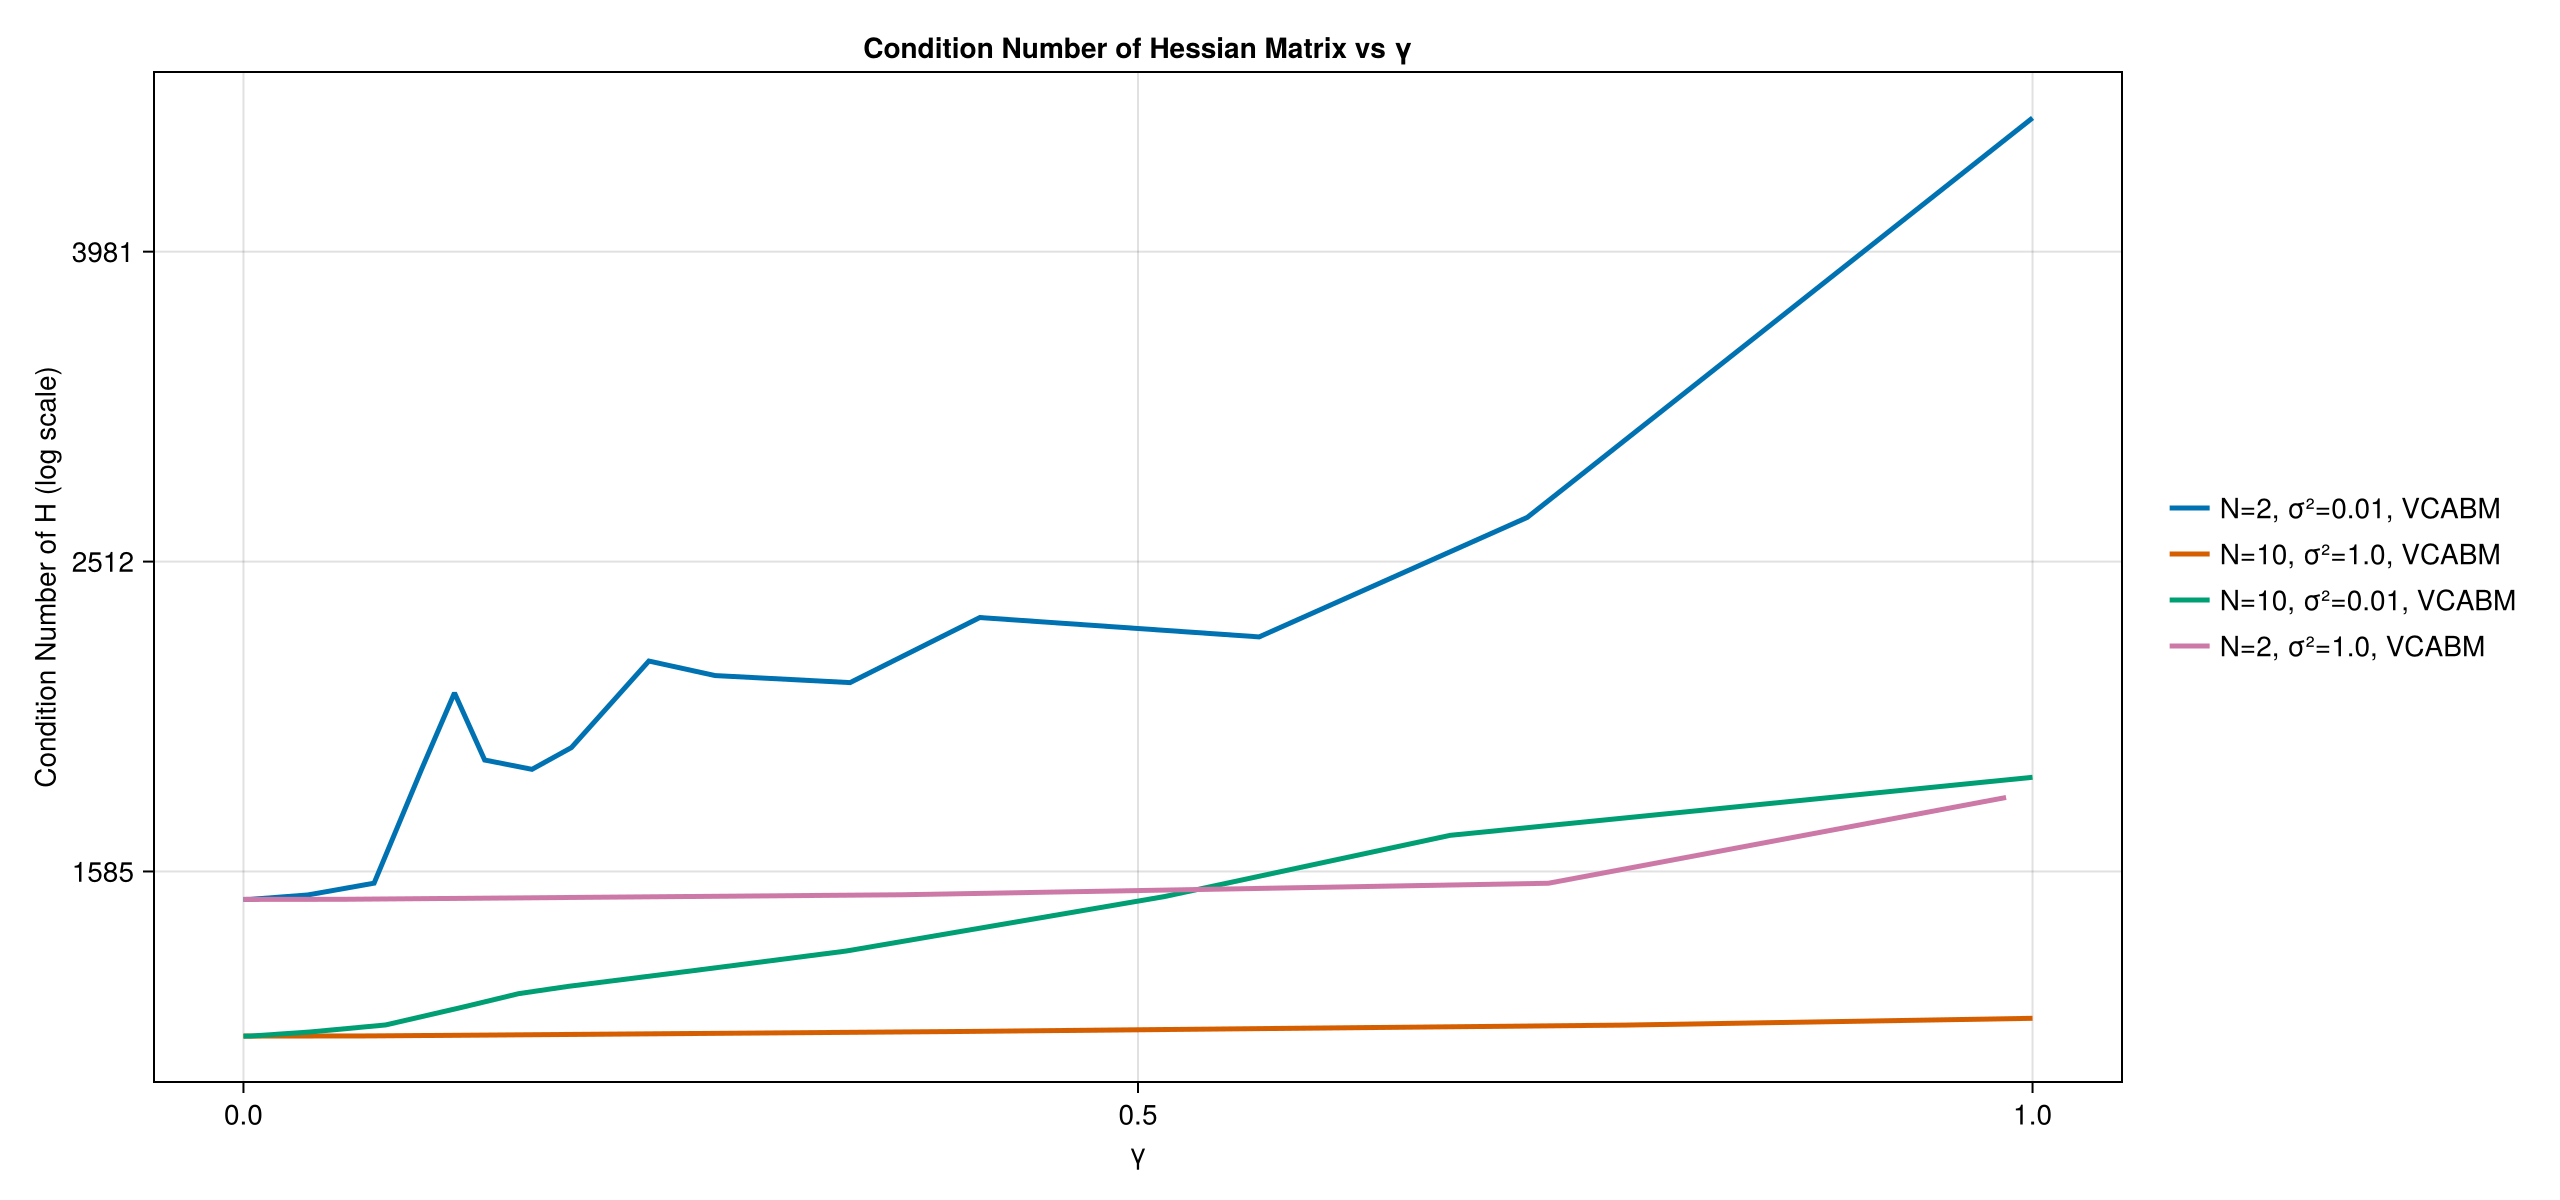
\includegraphics[width=0.9\textwidth]{./figures/condition_number_all.png}
	\caption{Condition number of matrix $\mH$.}
	\label{fig:condition_number}
\end{Figure}

% The results show that the condition number of $\mH$ generally remains below 3000. In addition, when the observation likelihood becomes narrower and the particles become more concentrated in space, the condition number increases accordingly.
To assess the numerical reliability of solving the linear system \(Ax=b\), it is useful to relate the condition number to the achievable accuracy. In finite-precision arithmetic, solving \(Ax=b\) typically loses about \(\log_{10}\kappa(A)\) decimal digits of accuracy. Therefore, a smaller condition number implies a more accurate numerical solution. Since the \texttt{Float64} type in Julia provides about 16 decimal digits of precision, the number of remaining significant digits can be approximated by
$\text{remaining significant digits} \approx 16 - \log_{10}\kappa(A)\enspace.$

\Fig{fig:condition_number} shows that the condition number of \(\mH\) generally remains below 3000. In addition, when the observation likelihood becomes narrower and the particles become more concentrated in space, the condition number increases accordingly. Since
$16 - \log_{10}(3000) \approx 12.5\enspace,$

the solution still retains about 12 significant digits even in the worst case considered here. Therefore, the numerical accuracy is more than sufficient for the MINRES solver tolerance of \(10^{-9}\), which confirms the practical feasibility of using MINRES in this study.

\begin{Figure}[ht]
	\centering
	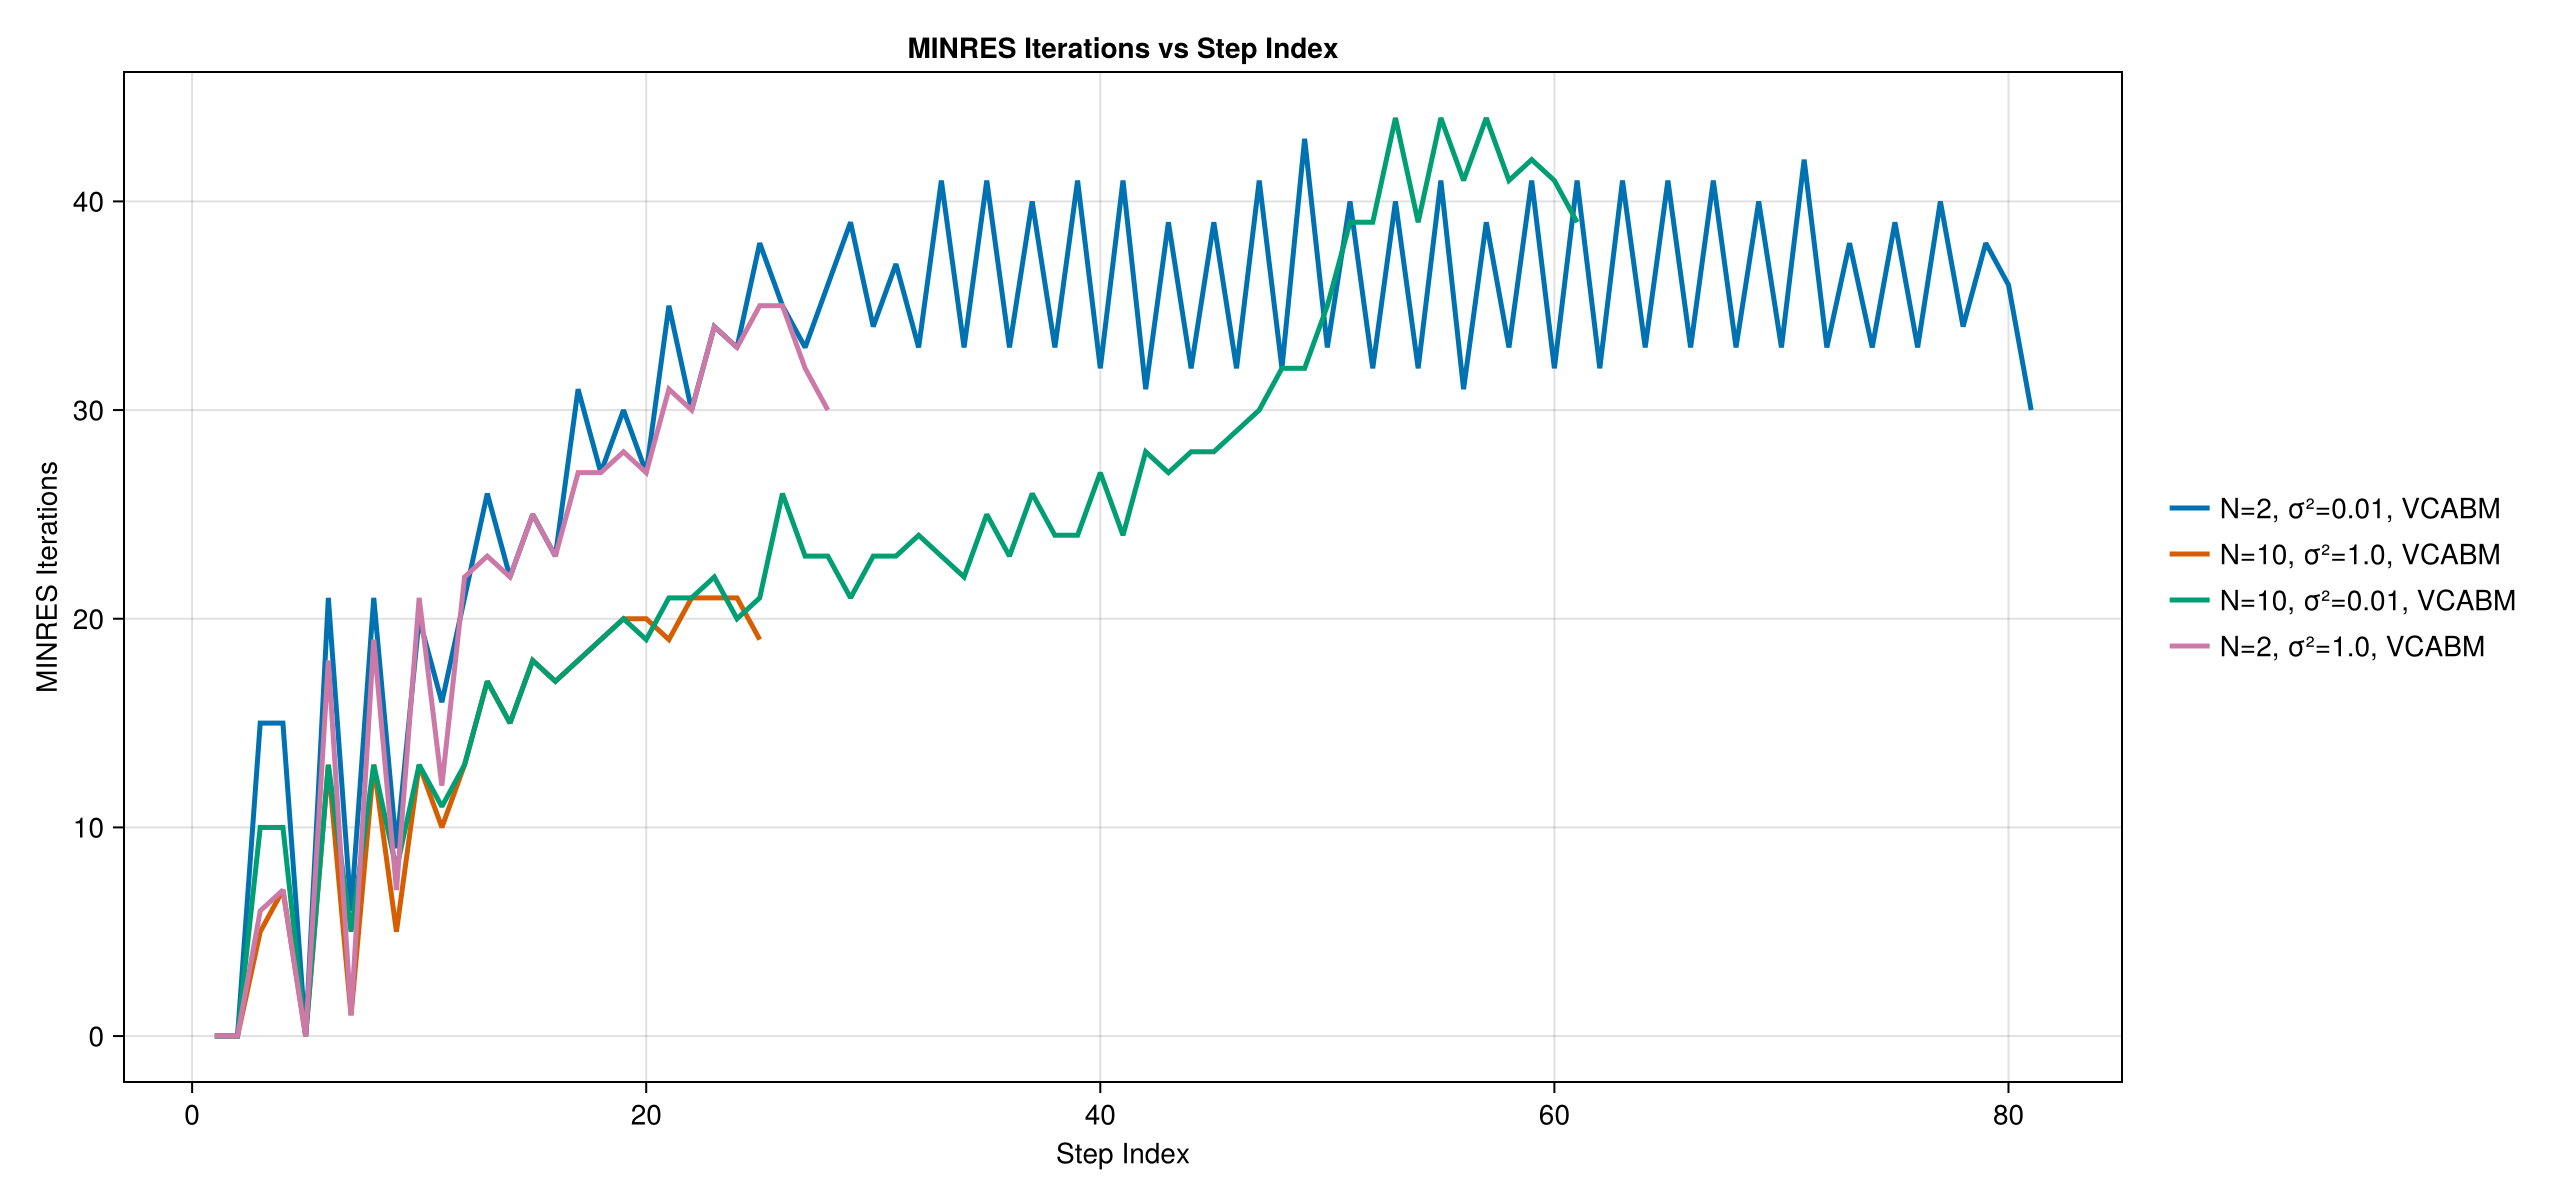
\includegraphics[width=0.9\textwidth]{./figures/minres_iterations_all.png}
	\caption{Number of iterations required for MINRES convergence.}
	\label{fig:minres_iterations}
\end{Figure}

Within the observed range of condition numbers, MINRES converges rapidly. In \Fig{fig:minres_iterations}, the iteration count $k$ usually does not exceed 50. Specifically, for a 2D system with 1000 particles (matrix dimension 2000), the relation $50 \ll \frac{2000}{3} \approx 667$ holds. For a 10D system with 1000 particles (matrix dimension 10000), the relation becomes $50 \ll \frac{10000}{3} \approx 3333$. These results demonstrate that MINRES is highly efficient for high-dimensional systems compared with Cholesky-based methods.

Furthermore, the iterative nature of MINRES naturally enables a warm-start strategy. When the integrator uses very small steps in $\gamma$, the changes in the system matrix $\mH$ and the vector $\mJ$ are also small. Therefore, this study uses the velocity $\dot{\eta}(\gamma^*)$ from the previous virtual-time step $\gamma^*$ as the initial guess for MINRES. Although the strict convergence tolerance ($10^{-9}$) limits the warm-start gain to only 1--2 iterations per call, the frequent use of MINRES during the integration of $\mH(\gamma)\dot{\eta}(\gamma) = -\mJ(\gamma)$ leads to a substantial cumulative reduction in the total number of matrix--vector products.

Since the Hessian matrix $\mH$ is symmetric and positive definite, the Conjugate Gradient (CG) method is also a viable option for solving the linear system. However, MINRES is preferred in this study because of its superior numerical stability while maintaining a computational speed comparable to that of CG.

\subsection{ODE Integrator Selection for Continuous Smooth Flow: The VCABM Method}
\label{subsec:vcabm}

When integrating the ODE $\mH(\gamma)\dot{\eta}(\gamma) = -\mJ(\gamma)$ from 0 to 1, the choice of numerical integrator depends mainly on the stiffness of the equation. If the system is highly stiff, even a small deviation of the particle position $\eta(\gamma)$ from the true trajectory can cause the evolution rate $\dot{\eta}(\gamma)$ to change sharply, making the numerical error grow rapidly \cite{NME}. To maintain stability, the integrator is then forced to use very small step sizes.

The stiffness of the ODE depends not only on the shape of the observation likelihood function $f_L(\vx)$, i.e., the variance of the measurement noise, but also on the geometric position of the particles relative to the likelihood. This dynamic relationship can be understood from the formula for the derivative of the true posterior weights with respect to virtual time
$$\dot{w}_i(\gamma)=\frac{\dot g(\gamma)\ln(f_L(\vx_i))}{L}-\frac{\sum_{j=1}^L \dot g(\gamma)\ln(f_L(\vx_j))}{L^2}\enspace.$$
Assuming a Gaussian observation likelihood, its log-likelihood $\ln(f_L(\vx))$ is geometrically a downward-opening parabola, or a high-dimensional paraboloid. The stiffness of the ODE depends on which region of this curve the particles occupy:

\textbf{Steep region far from the center (high stiffness):} If the prior particles are initially far from the effective likelihood region, they lie on the outer parts of the parabola. Since the outer regions of a quadratic function are steep, even a very small shift in the particle position $\vx_i$ causes a large change in $\ln(f_L(\vx_i))$. This sensitivity leads to a large variation in $\dot{w}_i(\gamma)$, which in turn induces significant changes in $\dot{\eta}$.

\textbf{Flat region near the center (low stiffness):} As virtual time progresses, the particles gradually flow toward the center of the likelihood, where the parabola becomes flatter. In this region, the log-likelihood is much less sensitive to small changes in particle position. Consequently, the value of $\dot{w}_i(\gamma)$ becomes more stable. Changes in the particle position $\eta$ no longer cause sharp jumps in $\dot{\eta}$, and the stiffness of the ODE decreases substantially.

This study uses the VCABM (Variable-Coefficient Adams--Bashforth--Moulton) multistep predictor--corrector integrator \cite{NME}. Its basic principle is as follows: at the beginning, the algorithm starts with small steps and collects sufficient historical information to construct a polynomial approximation. It then uses this polynomial to predict the particle position $\eta_{\mathrm{pre}}$ at the next virtual-time step and computes the flow rate $\dot{\eta}_{\mathrm{pre}}$ at the predicted point. Based on $\dot{\eta}_{\mathrm{pre}}$, the predictor is corrected to obtain the final value.

For highly stiff ODEs, even a slight deviation of the predicted position $\eta_{\mathrm{pre}}$ from the true trajectory can cause the computed flow rate $\dot{\eta}_{\mathrm{pre}}$ to become very large. This leads to a large discrepancy between the predicted and corrected values. If the discrepancy exceeds the tolerance, VCABM rejects the step and significantly reduces the step size $\Delta \gamma$ before retrying. In contrast, for weakly stiff ODEs, the predicted and corrected values remain close to each other, so the integrator can enlarge the step size and complete the integration more quickly.

To verify the suitability of VCABM, this study tests four cases in 2D and 10D systems($N=2,\enspace N=10$). In these experiments, the prior is a standard normal distribution, and the likelihood mean is $[3, 3, \dots]$. Likelihood variances of $\sigma^2 = 1.0$ (wide likelihood) and $\sigma^2 = 0.01$ (narrow likelihood) are used. Then use the VCABM integrator to calculate the integral value\Eq{eq:eta_flow_prior_posterior}. The experiments track the cumulative evolution of virtual time $\gamma$ as a function of the number of integration steps.

\begin{Figure}[ht]
	\centering
	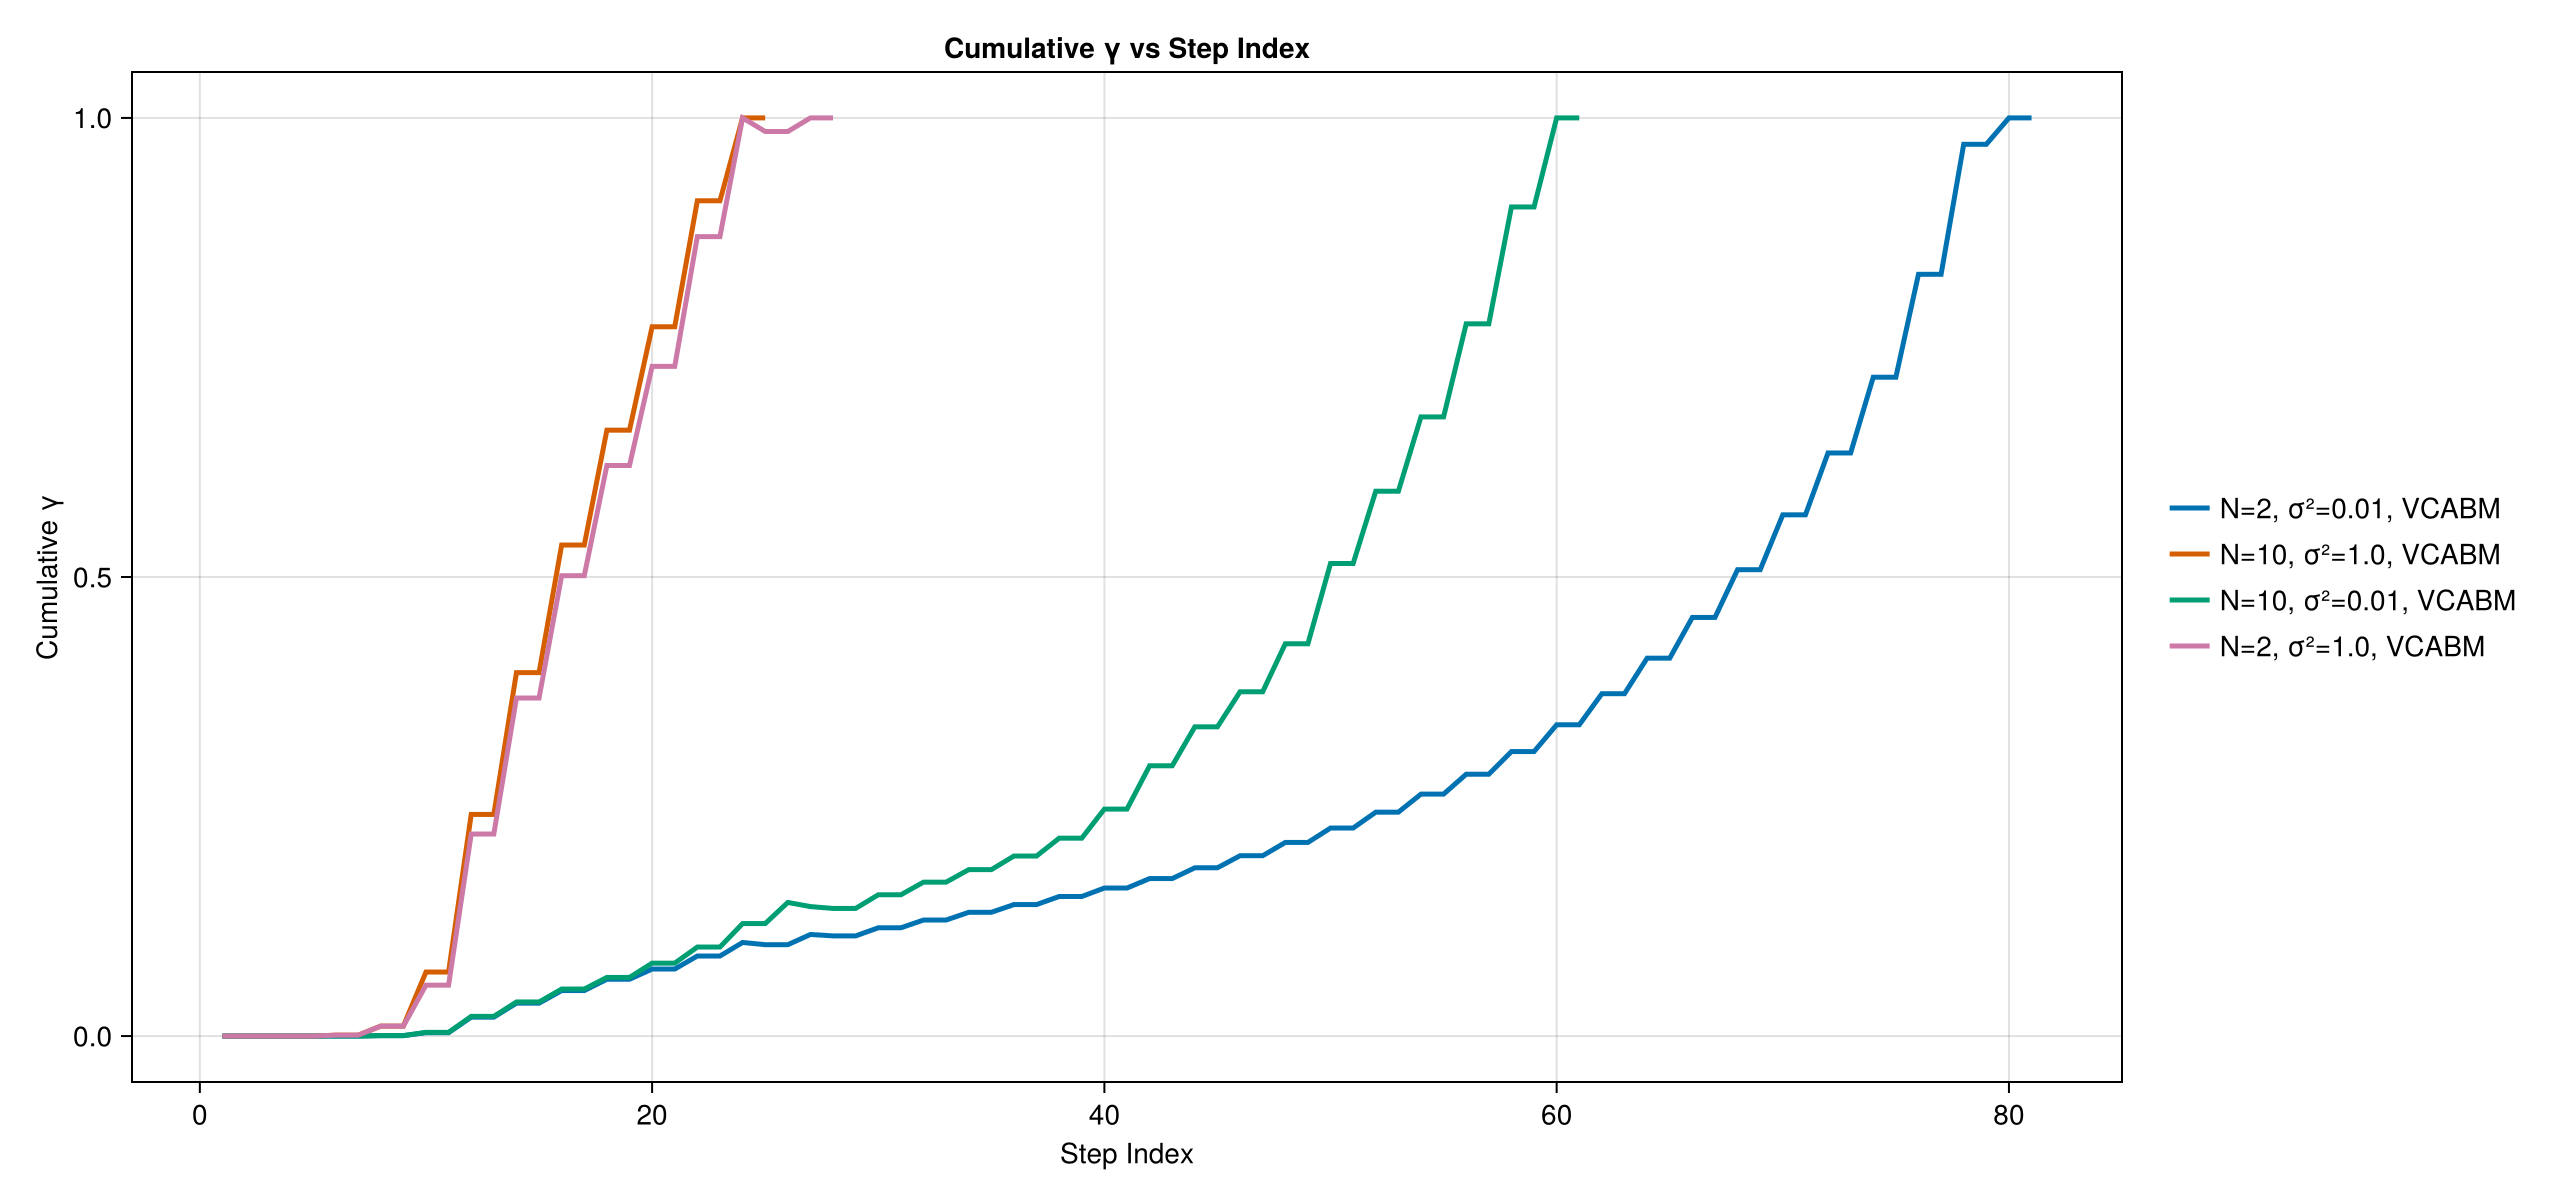
\includegraphics[width=0.85\textwidth]{./figures/cumulative_gamma_all.png}
	\caption{$\gamma$ vs. integration steps.}
	\label{fig:cumulative_gamma}
\end{Figure}

The experimental results in \Fig{fig:cumulative_gamma} agree with the theoretical analysis. When the likelihood variance is 1.0, the likelihood function is relatively flat, and the ODE stiffness remains low. VCABM can therefore use large step sizes consistently and completes the integration from $\gamma = 0$ to $1$ in fewer than 50 steps.

When the likelihood variance decreases to 0.01, the sharper likelihood function makes the ODE substantially stiffer. As a result, the integrator must use very small steps initially, increasing the total step count to around 100. Even though highly informative observations increase the numerical stiffness, the ODE remains within a regime that standard integrators can still handle effectively.

\section{Matrix-Free Method Based on MINRES}
\label{sec:matrix_free}

The implementation described above still requires storing the full Hessian matrix $\mH$ in GPU memory. However, storing the full Hessian introduces a severe memory bottleneck.

The dimension of $\mH$ is $NL \times NL$, so its memory requirement grows quadratically with both $N$ and $L$. For example, when $N=10$ and $L=2000$, the matrix $\mH$ has dimension $20000 \times 20000$. Using 64-bit floating-point numbers (\texttt{Float64}), this matrix alone occupies approximately 3.2~GB of GPU memory.

In practical engineering tests, parallel simulations are often required to evaluate the overall performance of the filter. If the system dimension and the particle number are increased further, or if multiple NFF instances run on the GPU simultaneously, this large matrix will quickly exhaust the available GPU memory. This leads to out-of-memory errors and makes large-scale parallel validation infeasible.

To overcome this bottleneck, the specific properties of MINRES can be exploited. As discussed in \Sec{subsec:minres}, during the iterative solution of $\mH\dot{\eta} = -\mJ$, MINRES does not need access to every individual element of $\mH$. Instead, it only requires the product of $\mH$ with an arbitrary vector $\vv$, i.e., the matrix--vector product $\mH\vv$.

Based on this fact, it is possible to avoid constructing and storing $\mH$ entirely. Instead, an analytical function can be derived that directly evaluates the product $\mH\vv$.

The matrix-free derivation of $\mH\vv$ is as follows.

For the $k$-th vector block $\vu_k$ (where $k \in \{1, 2, \dots, L\}$), the expression is
\begin{equation}
	\vu_k = (\mH\vv)_k = \sum_{j=1}^L \mH_{kj}\vv_j \enspace .
\end{equation}

Based on the blockwise form of the Hessian matrix in \Eq{eq:Hkl}, the off-diagonal and diagonal blocks can be treated in a unified way. Substituting $\mH_{kl} = 2w^2 \{ K\mI_N - 2\mathcal{H}(\vx_k - \vx_l) \}$ into the equation above yields
\begin{equation}
	\vu_k = 2w^2 \left( K \sum_{j=1}^L \vv_j - 2 \sum_{j=1}^L \mathcal{H}(\vx_k - \vx_j)\vv_j \right) \enspace .
\end{equation}

Substituting \Eq{eq:h} into the expression for $\vu_k$ and expanding it gives
\begin{equation}
	\vu_k = 2w^2 K \sum_{j=1}^L \vv_j - 8w^2 \sum_{j=1}^L \frac{2d_{\text{min}}^2 + \vd^{\top}\vd}{(d_{\text{min}}^2 + \vd^{\top}\vd)^2} \vd\vd^{\top} \vv_j - 4w^2 \sum_{j=1}^L \left[ \frac{\vd^{\top}\vd}{d_{\text{min}}^2 + \vd^{\top}\vd} + \log(d_{\text{min}}^2 + \vd^{\top}\vd) \right] \vv_j \enspace .
\end{equation}

By grouping similar terms, two scalar coefficients, $\alpha_{kj}$ and $\beta_{kj}$, can be defined as
\begin{align}
	\alpha_{kj} &= 2w^2 K - 4w^2 \frac{\vd^{\top}\vd}{d_{\text{min}}^2 + \vd^{\top}\vd} - 4w^2 \log(d_{\text{min}}^2 + \vd^{\top}\vd) \enspace , \\
	\beta_{kj} &= 8w^2 \frac{2d_{\text{min}}^2 + \vd^{\top}\vd}{(d_{\text{min}}^2 + \vd^{\top}\vd)^2} \enspace .
\end{align}

Using these two scalar coefficients, the expression for $\vu_k$ simplifies to
\begin{equation}
	\vu_k = \sum_{j=1}^L \alpha_{kj} \vv_j - \sum_{j=1}^L \beta_{kj} (\vd_{kj}^{\top} \vv_j) \vd_{kj} \enspace .
\end{equation}

If the second-moment penalty mechanism introduced earlier is included, the Hessian matrix becomes $\mH^{\mathrm{new}} = \mH^{\mathrm{original}} + \mH^{\mathrm{cov}}$, where the additional covariance block is
\begin{equation}
	\mH_{kl}^{\mathrm{cov}} = 4K_{\mathrm{cov}}w^2 \left( (\vx_k^{\top} \vx_l)\mI_N + \vx_l \vx_k^{\top} \right) \enspace .
\end{equation}
Accordingly,
\begin{equation}
	(\mH^{\mathrm{new}}\vv)_k = \vu_k^{\mathrm{original}} + \sum_{j=1}^L 4K_{\mathrm{cov}}w^2 \left( (\vx_k^{\top} \vx_j)\vv_j + (\vx_k^{\top} \vv_j)\vx_j \right) \enspace .
\end{equation}

MINRES typically requires tens of iterations, meaning that the matrix-free product $\mH\vv$ must be evaluated many times. However, the scalars $\alpha_{kj}$ and $\beta_{kj}$ depend only on the particle positions $\vx$ at the current virtual time and therefore remain constant during a single MINRES solve.

Therefore, when computing the vector $\mJ$, the coefficients $\alpha_{kj}$ and $\beta_{kj}$ can be precomputed and stored in two $L \times L$ scalar matrices $\mA$ and $\mB$, where $\mA_{kj} = \alpha_{kj}$ and $\mB_{kj} = \beta_{kj}$. In the subsequent MINRES iterations, the algorithm no longer needs to recompute the expensive kernel expressions. Instead, it only performs matrix lookups, dot products, and vector operations. This matrix-free scheme reduces the memory complexity from $O((NL)^2)$ to $O(L^2)$.

\section{NFF Prediction Step}
\label{sec:prediction_step}

The previous sections described the update step of NFF. However, a complete nonlinear filtering procedure also requires a prediction step. This study implements the following three prediction methods.

\subsection{Method 1}
\label{subsec:method1}

The first prediction mechanism is identical to the prediction step used in PF. For the $L$ posterior particles obtained after the update step at time $k-1$, the algorithm draws a random noise sample $\vv_{k-1}^{(i)}$ from the process noise distribution $\mathcal{N}(\mathbf{0}, \mQ)$ for each particle $\vx_{k-1}^{(i)}$.

Each particle is then propagated by one step through the discretized system evolution equation together with its corresponding noise sample, yielding $L$ new prior particles given by
\begin{equation}
	\vx_k^{(i)} = f_k(\vx_{k-1}^{(i)}, \vv_{k-1}^{(i)}), \quad i = 1, 2, \dots, L \enspace .
\end{equation}

\subsection{Method 2}
\label{subsec:method2}

The second prediction method begins by deterministically extracting $K$ fixed noise samples $\vv_{k-1}^{(j)}$ ($j = 1, 2, \dots, K$) from the process noise distribution $\mathcal{N}(\mathbf{0}, \mQ)$. Next, each posterior particle from the previous time step is combined with all $K$ noise samples and propagated forward. This is equivalent to taking the Cartesian product of the state particles and the noise samples, resulting in a total of $L \times K$ predicted points using
\begin{equation}
	\vx_k^{(i,j)} = f_k(\vx_{k-1}^{(i)}, \vv_{k-1}^{(j)}), \quad i = 1, \dots, L, \quad j = 1, \dots, K \enspace ,
\end{equation}
where $\vx_{k-1}^{(i)}$ denotes the $i$-th posterior particle at time $k-1$. After generating this set of $L \times K$ points, the algorithm applies an optimal reduction procedure. This procedure treats the $L \times K$ points as a fixed reference distribution and optimizes $L$ equally weighted particles by minimizing the modified \ac{cvm} between the optimized set and the reference set. The resulting $L$ particles serve as the prior distribution at the current time step.

\begin{Figure}[ht]
	\centering
	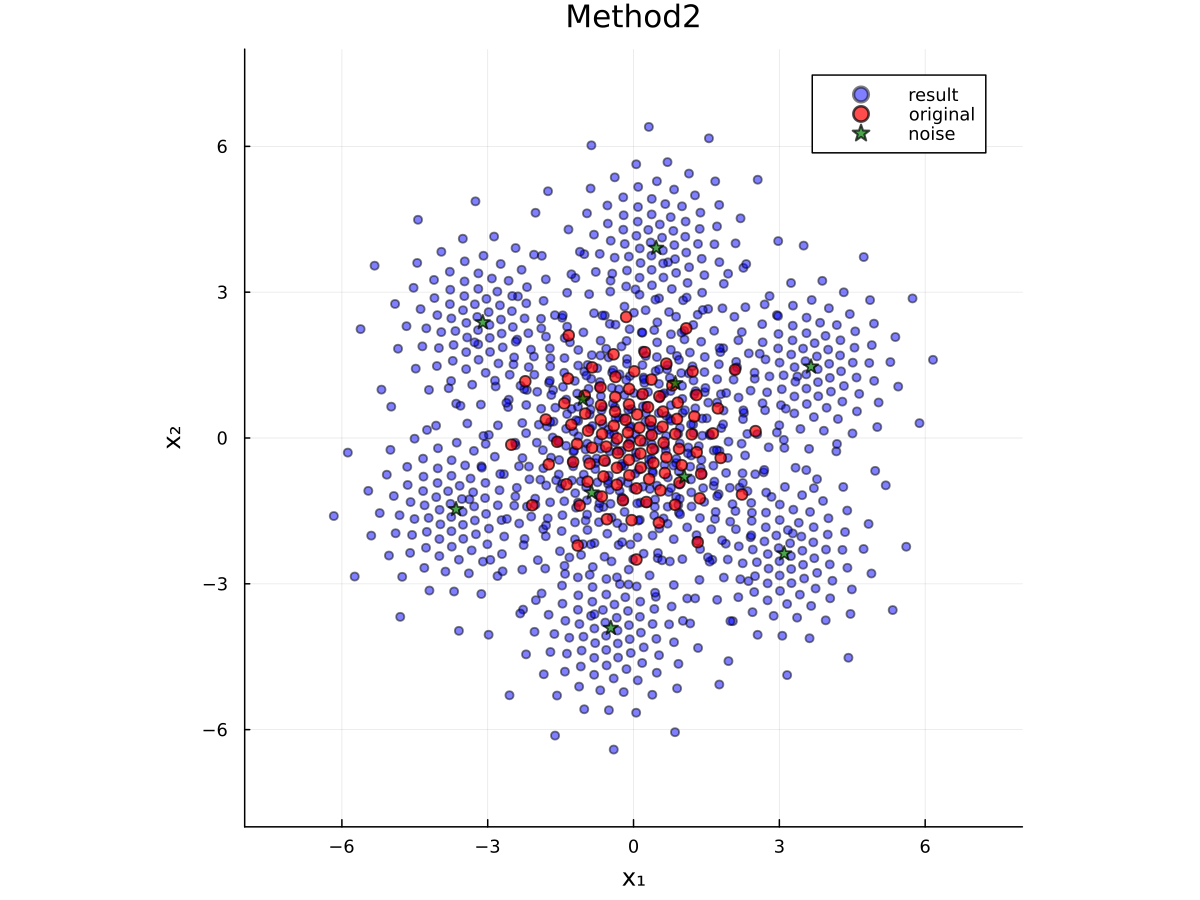
\includegraphics[width=0.9\textwidth]{figures/Examples/method2_final.png}
	\caption{Visualization of Method 2.}
	\label{fig:method2_viz}
\end{Figure}
\clearpage

\subsection{Method 3}
\label{subsec:method3}

In this method, the algorithm concatenates the $L$ particles of dimension $N$ from the current posterior into a single high-dimensional particle of dimension $L \times N$. At the same time, the process noise distribution is lifted to an $L \times N$-dimensional Gaussian distribution
\[
\mathcal{N}(\mathbf{0}, \text{diag}(\mQ, \dots, \mQ)) \enspace ,
\]
whose covariance is block diagonal with $L$ copies of $\mQ$.

In this high-dimensional noise space, the algorithm deterministically extracts $K$ high-dimensional noise samples $\vv_{k-1}^{(j)}$ ($j = 1, 2, \dots, K$). The current high-dimensional particle is then propagated through the system equations using each of these $K$ noise samples, yielding $K$ high-dimensional particles given by
\begin{equation}
	\begin{bmatrix} \vx_k^{(1, j)} \\ \vdots \\ \vx_k^{(L, j)} \end{bmatrix} = \begin{bmatrix} f_k(\vx_{k-1}^{(1)}, \vv_{k-1}^{(j, 1)}) \\ \vdots \\ f_k(\vx_{k-1}^{(L)}, \vv_{k-1}^{(j, L)}) \end{bmatrix}, \quad j = 1, 2, \dots, K \enspace ,
\end{equation}
where $\vv_{k-1}^{(j, i)}$ denotes the components of the $j$-th high-dimensional noise sample from dimension $(i-1)N + 1$ to $iN$.

After obtaining these $K$ high-dimensional particles, each one is split into $L$ separate $N$-dimensional particles. In this way, the $K$ super-particles are effectively transformed into $K \times L$ particles of dimension $N$. Finally, the optimal reduction algorithm reduces these $K \times L$ particles back to $L$ particles, thereby completing the prediction step.

\begin{Figure}[ht]
	\centering
	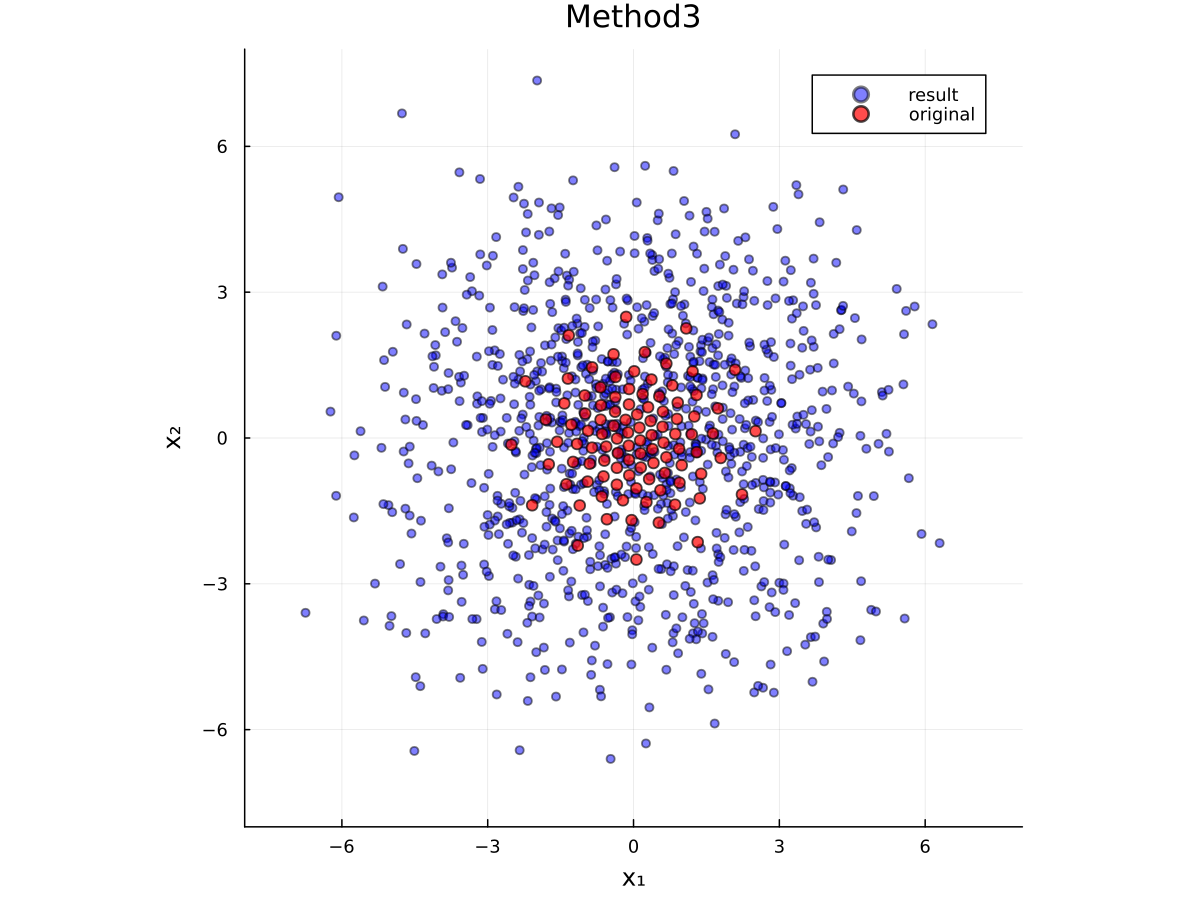
\includegraphics[width=0.8\textwidth]{figures/Examples/method1_final.png}
	\caption{Visualization of Method 3.}
	\label{fig:method3_viz}
\end{Figure}

\clearpage

\subsection{Prediction Step for the Lorenz 96 System}
\label{subsec:lorenz96_prediction}

When discretizing the Lorenz 96 system, the total perturbation over the macroscopic integration step $\Delta t$ must first be determined. For the stochastic noise term in the system equation, this requires integrating the standard Wiener process increment $d\mW_t$ over the interval $[t_{k-1}, t_k]$ as
\begin{equation}
	\vv_{k-1} = \int_{t_{k-1}}^{t_k} \mG d\mW_t \enspace .
\end{equation}
The multidimensional standard Wiener process can be interpreted as follows: at every infinitesimal time interval $dt$, the system is perturbed by an independent Gaussian increment $\Gaussian(\vzero, \mI dt)$ with an infinitesimal covariance. Integrating the Wiener process over an interval of length $\Delta t$ amounts to a continuous superposition of infinitely many independent Gaussian increments. By the additivity of independent Gaussian random variables, the sum remains Gaussian, and the total covariance equals the sum of the infinitesimal covariances, i.e., $\sum \mI dt = \mI \Delta t$. Therefore, over the macroscopic step $\Delta t$, the cumulative process noise $\vv_{k-1}$ follows
\begin{equation}
	\vv_{k-1} \sim \Gaussian\left(\vzero, \Delta t \mG \mG^{\top}\right) \enspace .
\end{equation}

In Method 1 described in \Sec{subsec:method1}, the algorithm uses purely stochastic sampling. To simulate the Lorenz 96 system accurately, Method 1 adopts the standard Euler--Maruyama (EM) scheme. EM divides the macroscopic step $\Delta t$ into $M$ microscopic substeps of size $dt = \Delta t / M$. At each microscopic time step $m$, the algorithm generates a new independent Gaussian increment $\Delta \mW_m \sim \Gaussian(\vzero, \mI dt)$ and updates the state according to
\begin{equation}
	\vx_{m+1} = \vx_m + \vf(\vx_m)dt + \mG\Delta \mW_m \quad (m = 0, 1, \dots, M-1) \enspace .
\end{equation}
Since the increments $\Delta \mW_m$ are mutually independent, after $M$ steps the accumulated variance becomes $M \times dt \mG\mG^{\top} = \Delta t \mG\mG^{\top}$.

When deterministic sampling is introduced in Method 2 and Method 3, the algorithm must deterministically extract $K$ sample points $\vv^{(k)}$ ($k = 1, 2, \dots, K$) from the macroscopic process noise distribution $\Gaussian(\vzero, \Delta t \mG\mG^{\top})$. At this point, a common engineering pitfall arises. If one propagates the particles over $\Delta t$ using only the drift term $\vf(\vx_t)$ and then simply adds the extracted macroscopic noise samples $\vv^{(k)}$ afterward, this procedure completely ignores the continuous influence of the stochastic term on the nonlinear trajectory during the interval $\Delta t$.

To address this issue, this study replaces the stochastic EM paths with deterministic straight-line paths. In the standard Euler--Maruyama method, the noise path starts at $\vzero$ and ends at a random sample drawn from $\Gaussian(\vzero, \Delta t \mG\mG^{\top})$. Here, by contrast, each deterministically extracted macroscopic noise sample $\vv^{(k)}$ is interpreted as a straight-line path from $\vzero$ to $\vv^{(k)}$ in the noise space. Across the $M$ microscopic substeps, the algorithm injects the incremental component of this path, i.e., $\frac{\vv^{(k)}}{M}$, at each step. The update formula becomes
\begin{equation}
	\tilde{\vx}_{m+1} = \tilde{\vx}_m + \vf(\tilde{\vx}_m) dt + \frac{\vv^{(k)}}{M} \qquad (m = 0, 1, \dots, M-1) \enspace .
\end{equation}
After $M$ microscopic steps, the final propagated state is $\vx_{t+\Delta t} = \tilde{\vx}_M$. In this way, each prior particle evolves along $K$ different deterministic straight-line paths. Because the noise is injected throughout the nonlinear integration process, the dynamic coupling between the stochastic term and the system evolution is effectively preserved.

\begin{Figure}[ht]
	\centering
	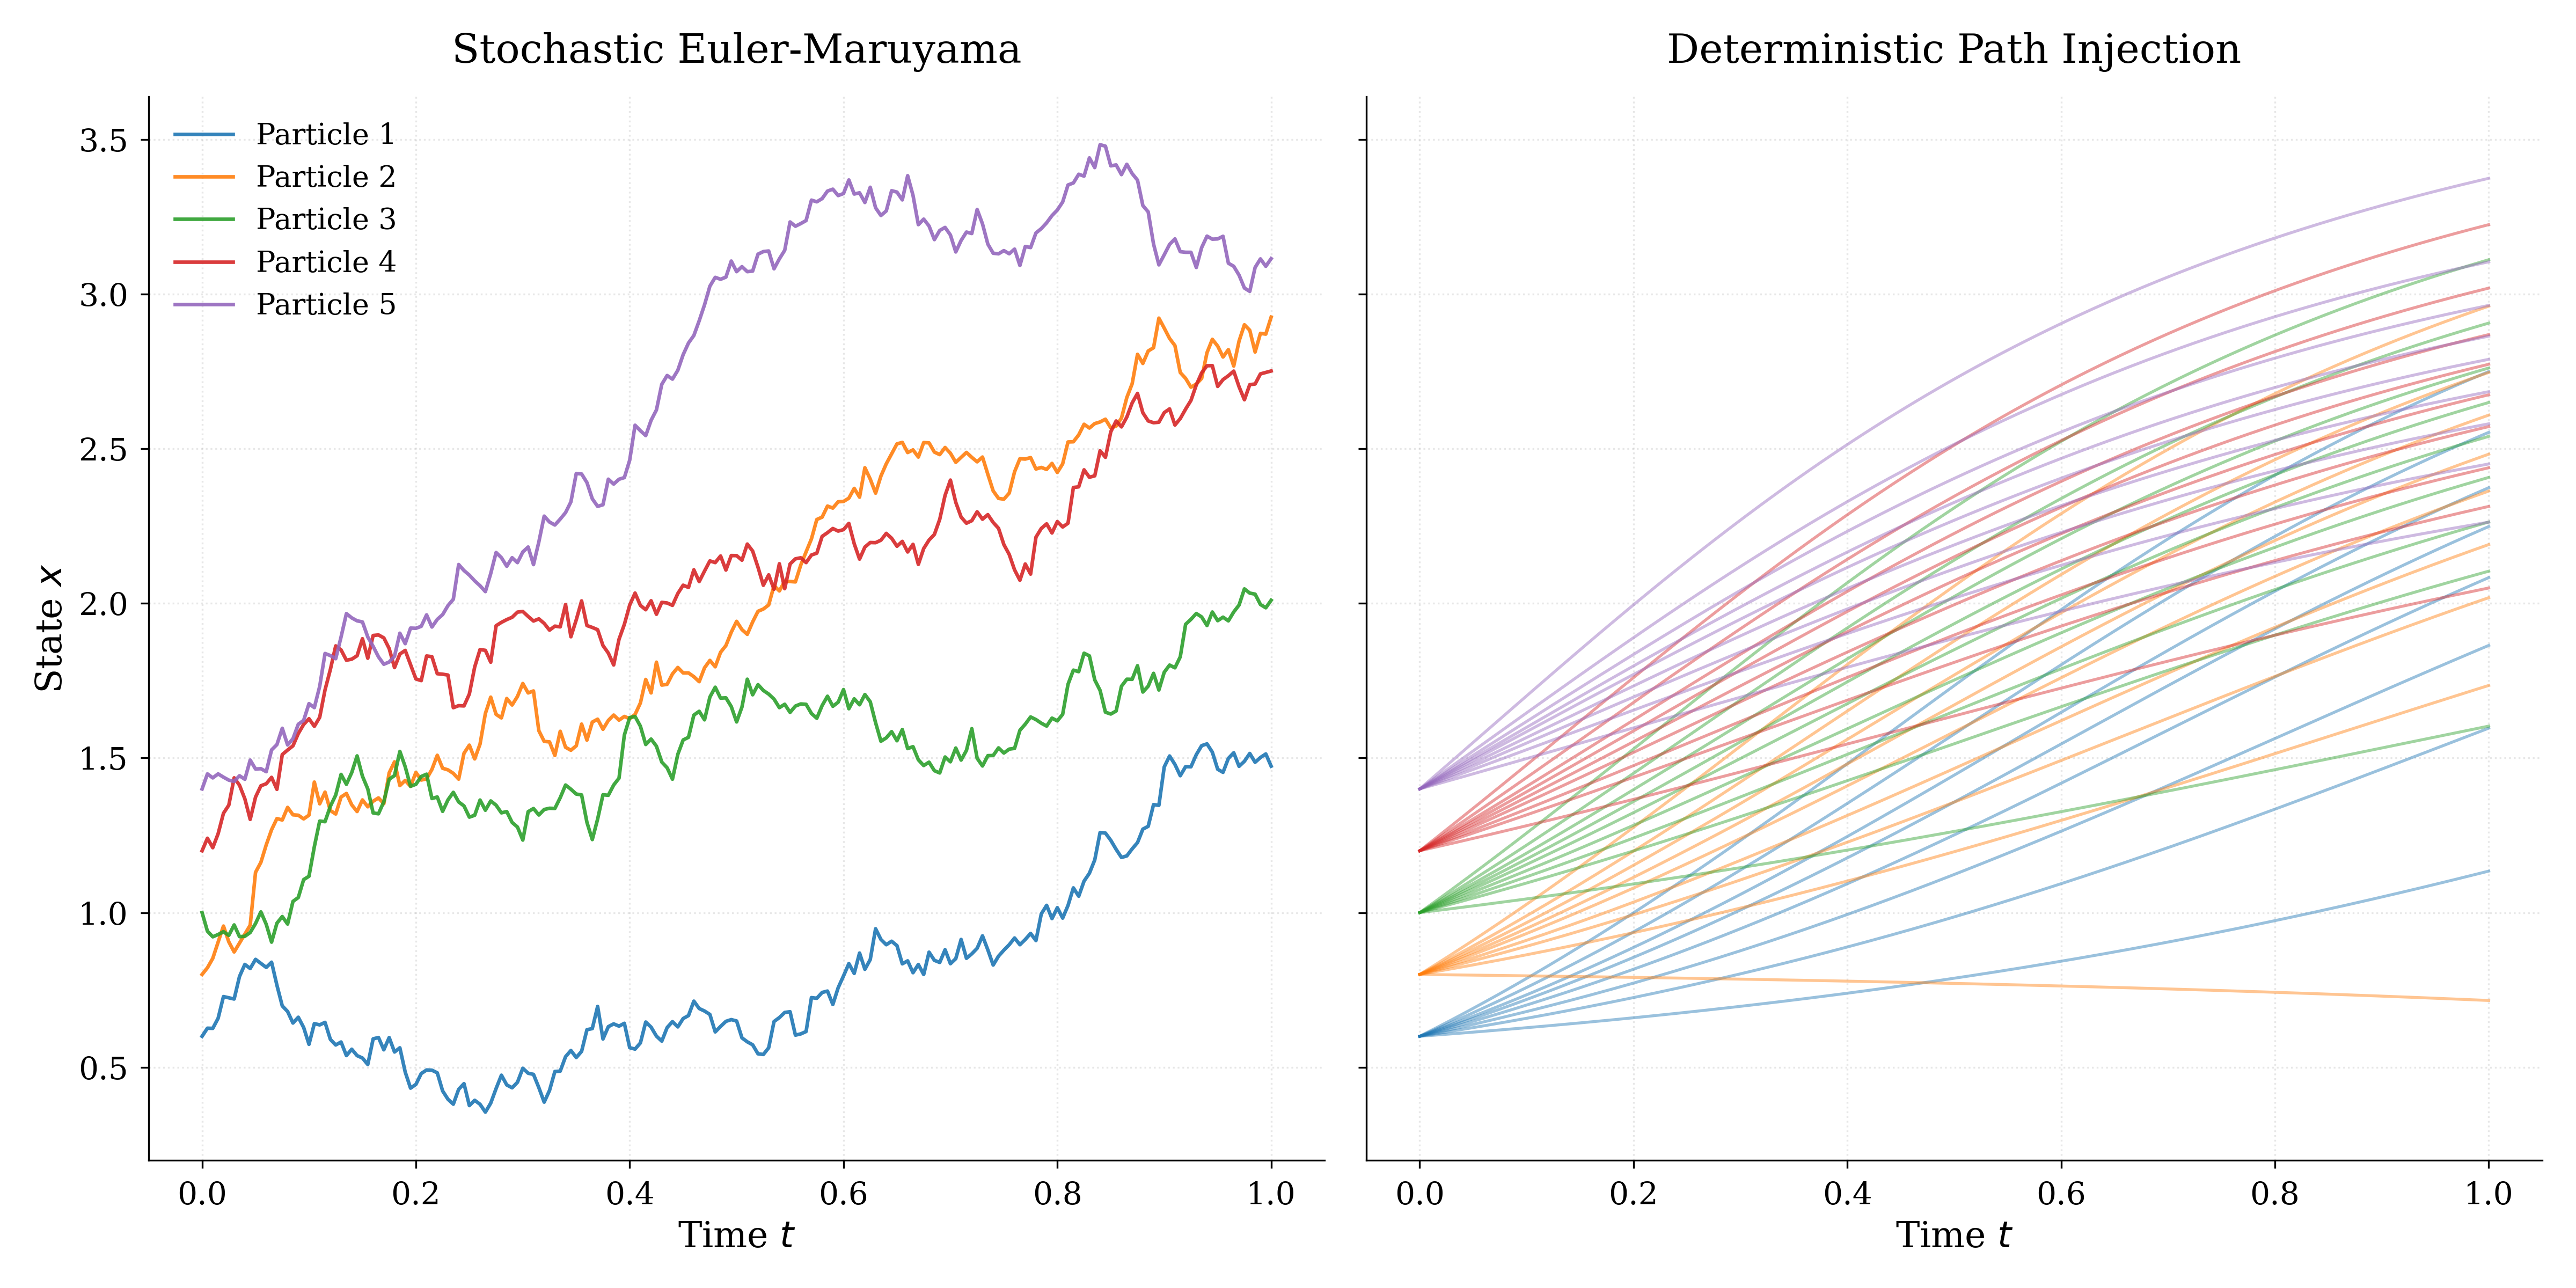
\includegraphics[width=0.95\textwidth]{figures/nonlinear_comparison.png}
	\caption{Comparison of noise injection strategies in the prediction step. }
	\label{fig:sde_comparison}
\end{Figure}

As shown in the \Fig{fig:sde_comparison}, the deterministic noise injection method enables a more uniform exploration of the state space, thereby capturing significantly more predictive information.

Within this straight-line path framework, the main difference between Method 2 and Method 3 lies in the independence of the paths. In Method 2, deterministic sampling is performed in a low-dimensional space, so all $L$ particles share the same $K$ straight-line evolution paths. In Method 3, deterministic sampling is performed in an extremely high-dimensional space, so each particle has its own set of $K$ exclusive straight-line evolution paths, completely independent of those of the other particles.

\subsection{Numerical Overflow and Acceleration Strategies for High-Dimensional Deterministic Sampling}
\label{subsec:overflow_strategies}

In Method 3 described in \Sec{subsec:method3}, deterministic sampling must be performed in a space of dimension $N \times L$, which is typically greater than 10,000. This is done by minimizing the modified Cramér--von Mises distance between a Gaussian distribution and a Dirac mixture distribution \cite{LCDSM}. However, when evaluating the distance $D$ and its gradient $G$ in such high dimensions, serious numerical overflow and efficiency bottlenecks arise.

According to Dirac mixture approximation theory for multivariate Gaussian distributions, the modified CVM distance $D$ between a Gaussian distribution $\tilde{f}$ and a Dirac mixture $f$ can be decomposed into three parts as
\begin{equation}
	D = D_1 - 2D_2 + D_3, \quad \text{where} \quad D_i = \int_0^{b_{\max}} \frac{1}{b^{N-1}} P_i \dd b \quad (i = 1, 2, 3) \enspace .
\end{equation}
Here, $D_1$ is a constant independent of the Dirac mixture and can therefore be ignored during optimization. The expressions for $P_2$ and $D_3$ are
\begin{equation}
	P_2 = (2\pi)^{\frac{N}{2}} b^{2N} \left( \prod_{k=1}^N \frac{1}{\sqrt{(\sigma^{(k)})^2 + 2b^2}} \right) \sum_{i=1}^L w_i \exp\!\left( -\frac{1}{2} \sum_{k=1}^N \frac{(x_i^{(k)})^2}{(\sigma^{(k)})^2 + 2b^2} \right) \enspace ,
\end{equation}
\begin{equation}
	D_3 = \frac{\pi^{\frac{N}{2}}}{8} \sum_{i=1}^L \sum_{j=1}^L w_i w_j \Big( 4b_{\max}^2 - C_b T_{ij} + T_{ij}\log(T_{ij}) \Big) \enspace ,
\end{equation}
where $T_{ij} = \sum_{k=1}^N (x_i^{(k)} - x_j^{(k)})^2$ and the constant $C_b = \log(4b_{\max}^2) - \Gamma$. To determine the optimal particle locations $\vx$ that minimize the distance, the partial derivative of the distance function with respect to the $\eta$-th component of the $\xi$-th particle, $x_\xi^{(\eta)}$, is derived as $G_\xi^{(\eta)} = G_\xi^{(\eta, 1)} + G_\xi^{(\eta, 2)}$, where
\begin{equation}
\begin{split}
    G_\xi^{(\eta, 1)} = {} & 2(2\pi)^{\frac{N}{2}} w_\xi x_\xi^{(\eta)} \int_0^{b_{\text{max}}} \frac{b^{N+1}}{(\sigma^{(\eta)})^2 + 2b^2} \left( \prod_{k=1}^N \frac{1}{\sqrt{(\sigma^{(k)})^2 + 2b^2}} \right) \text{\raisebox{-.7\baselineskip}[0pt][0pt]{\rotatebox[origin=c]{180}{$\Rsh$}}} \\
    & \exp\!\left( -\frac{1}{2} \sum_{k=1}^N \frac{(x_\xi^{(k)})^2}{(\sigma^{(k)})^2 + 2b^2} \right) \dd b \enspace ,
\end{split}
\end{equation}
\begin{equation}
	G_\xi^{(\eta, 2)} = \frac{\pi^{\frac{N}{2}}}{2} w_\xi \left\{ \sum_{i=1}^L w_i (x_\xi^{(\eta)} - x_i^{(\eta)}) \log\left( \sum_{k=1}^N (x_\xi^{(k)} - x_i^{(k)})^2 \right) + C_b \left( \sum_{i=1}^L w_i x_i^{(\eta)} - x_\xi^{(\eta)} \right) \right\} \enspace .
\end{equation}

As shown above, the terms $D_2$, $D_3$, and the gradients $G^{(1)}$, $G^{(2)}$ all contain the constant factor $\pi^{N/2}$. Since this factor does not affect the optimizer, it can be omitted during optimization.

When the dimension $N$ reaches 10,000, terms such as $b^{N+1}$ in the integral cause severe numerical overflow. To handle this problem, this study applies a logarithmic transformation. Using this log trick, the powers and products in the kernel of the $D_2$ integral are rewritten in the form $\exp(\ln(\cdot))$ as
\begin{equation}
	\begin{split}
		D_2 = \int_0^{b_{\text{max}}} &\exp\!\left( (N+1)\ln b + \frac{N}{2}\ln 2 - \sum_{k=1}^N \frac{1}{2} \ln((\sigma^{(k)})^2 + 2b^2) \right) \text{\raisebox{-.7\baselineskip}[0pt][0pt]{\rotatebox[origin=c]{180}{$\Rsh$}}} \\
		&\cdot \sum_{i=1}^L w_i \exp\!\left( -\frac{1}{2} \sum_{k=1}^N \frac{(x_i^{(k)})^2}{(\sigma^{(k)})^2 + 2b^2} \right) \dd b \enspace .
	\end{split}
\end{equation}

Similarly, for the gradient term $G_\xi^{(\eta, 1)}$, after factoring out the external constants, the integral kernel can be rewritten in a numerically safe form as
\begin{equation}
	\begin{split}
		G_\xi^{(\eta, 1)} \propto \int_0^{b_{\text{max}}} & \exp\! \bigg( (N+1)\ln b + \left(\frac{N}{2}+1\right)\ln 2 - \ln((\sigma^{(\eta)})^2 + 2b^2) \text{\raisebox{-.7\baselineskip}[0pt][0pt]{\rotatebox[origin=c]{180}{$\Rsh$}}} \\
		& - \sum_{k=1}^N \frac{1}{2} \ln((\sigma^{(k)})^2 + 2b^2) \bigg) \cdot \exp\!\left( -\frac{1}{2} \sum_{k=1}^N \frac{(x_\xi^{(k)})^2}{(\sigma^{(k)})^2 + 2b^2} \right) \dd b \enspace .
	\end{split}
\end{equation}

In the implementation, the logarithmic terms are summed first. Because the large positive contribution from $(N+1)\ln b$ is offset by the large negative contribution from $-\sum \frac{1}{2}\ln(\cdot)$, the final exponent remains within a numerically stable range and avoids overflow.

Sampling $K$ points in a space of dimension $N \times L$ requires $N \times L \times K$ integration operations in each optimization step. For a problem of this scale, adaptive numerical integration would be prohibitively slow.

Therefore, this study uses a fixed-point integration scheme in the implementation. This method approximates the continuous integral by a finite weighted sum via
\begin{equation}
	\int f(b) \dd b \approx \sum_{i=1}^M c_i f(b_i) \enspace .
\end{equation}

To verify the performance of the three prediction mechanisms under different dimensions and noise conditions, as well as the feasibility of the improved LCD sampling code, a set of basic state-propagation experiments is designed. The discrete state transition equation used in the experiments is
\begin{equation}
	\vx_k = \vx_{k-1} + \vv_{k-1} \enspace ,
\end{equation}
where the posterior particles $\vx_{k-1}$ from the previous step are obtained by deterministic sampling from a standard normal distribution $\mathcal{N}(\mathbf{0}, \mI)$.

The experiments are conducted in low-dimensional settings (2D, $L=100$ particles) and high-dimensional settings (10D, $L=1000$ particles). Different process noise variances $\sigma^2 \in \{1.0, 2.0, 5.0, 10.0\}$ are also tested. The mean and covariance of the prior particles generated by the three prediction methods are compared with the true analytical solution, i.e., $\mathcal{N}(\mathbf{0}, \mI + \sigma^2\mI)$. The results are shown in \Tab{tab:cov_error} and \Tab{tab:mean_error}.

\begin{Table}[ht]
	\centering
	\small
	\begin{tabular}{|c|c|c|c|c|c|c|}
		\hline
		System Dim. & $\sigma^2$ & \multicolumn{3}{c|}{Method 1 (Stochastic)} & Method 2 & Method 3 \\ \cline{3-5}
		& & $L_{\mathrm{noise}}=10$ & $L_{\mathrm{noise}}=20$ & $L_{\mathrm{noise}}=50$ & ($L_{\mathrm{noise}}=10$) & ($L_{\mathrm{noise}}=10$) \\ \hline
		\textbf{2D}  & 1.0  & 0.0569 & 0.1013 & 0.0296 & \textbf{0.0035} & 0.0681 \\ \cline{2-7}
		($L=100$)    & 2.0  & 0.0658 & 0.1617 & 0.0606 & \textbf{0.0070} & 0.1362 \\ \cline{2-7}
		& 5.0  & 0.0843 & 0.3254 & 0.1576 & \textbf{0.0174} & 0.3406 \\ \cline{2-7}
		& 10.0 & 0.1673 & 0.5860 & 0.3236 & \textbf{0.0347} & 0.6812 \\ \hline
		\textbf{10D} & 1.0  & 0.1746 & \textbf{0.0996} & --     & 2.2350 & 0.1098 \\ \cline{2-7}
		($L=1000$)   & 2.0  & 0.2868 & \textbf{0.1648} & --     & 4.4700 & 0.2193 \\ \cline{2-7}
		& 5.0  & 0.6056 & \textbf{0.3644} & --     & 11.1750 & 0.5478 \\ \cline{2-7}
		& 10.0 & 1.1287 & \textbf{0.7094} & --     & 22.3500 & 1.0953 \\ \hline
	\end{tabular}
	\caption{Comparison of RFE\Eq{eq:Rfe} for different prediction mechanisms.}
	\label{tab:cov_error}
\end{Table}

\begin{Table}[ht]
	\centering
	\small
	\begin{tabular}{|c|c|c|c|c|c|c|}
		\hline
		System & Proc. Noise & \multicolumn{3}{c|}{Method 1 (Stochastic)} & Method 2 & Method 3 \\ \cline{3-5}
		Dim. & Var. ($\sigma^2$) & $L_{\mathrm{noise}}=10$ & $L_{\mathrm{noise}}=20$ & $L_{\mathrm{noise}}=50$ & ($L_{\mathrm{noise}}=10$) & ($L_{\mathrm{noise}}=10$) \\ \hline
		\textbf{2D}  & 1.0  & $1.63 \times 10^{-2}$ & $2.29 \times 10^{-2}$ & $1.93 \times 10^{-2}$ & $\bm{3.43 \times 10^{-6}}$ & $\bm{3.43 \times 10^{-6}}$ \\ \cline{2-7}
		($L=100$)    & 2.0  & $2.31 \times 10^{-2}$ & $3.24 \times 10^{-2}$ & $2.74 \times 10^{-2}$ & $\bm{3.43 \times 10^{-6}}$ & $\bm{3.43 \times 10^{-6}}$ \\ \cline{2-7}
		& 5.0  & $3.65 \times 10^{-2}$ & $5.12 \times 10^{-2}$ & $4.33 \times 10^{-2}$ & $\bm{3.43 \times 10^{-6}}$ & $\bm{3.43 \times 10^{-6}}$ \\ \cline{2-7}
		& 10.0 & $5.16 \times 10^{-2}$ & $7.24 \times 10^{-2}$ & $6.12 \times 10^{-2}$ & $\bm{3.42 \times 10^{-6}}$ & $3.43 \times 10^{-6}$ \\ \hline
		\textbf{10D} & 1.0  & $3.68 \times 10^{-2}$ & $2.48 \times 10^{-2}$ & --     & $7.54 \times 10^{-6}$ & $\bm{7.53 \times 10^{-6}}$ \\ \cline{2-7}
		($L=1000$)   & 2.0  & $5.20 \times 10^{-2}$ & $3.51 \times 10^{-2}$ & --     & $7.54 \times 10^{-6}$ & $\bm{7.53 \times 10^{-6}}$ \\ \cline{2-7}
		& 5.0  & $8.22 \times 10^{-2}$ & $5.54 \times 10^{-2}$ & --     & $7.54 \times 10^{-6}$ & $\bm{7.53 \times 10^{-6}}$ \\ \cline{2-7}
		& 10.0 & $1.16 \times 10^{-1}$ & $7.84 \times 10^{-2}$ & --     & $7.55 \times 10^{-6}$ & $\bm{7.53 \times 10^{-6}}$ \\ \hline
	\end{tabular}
	\caption{Comparison of mean error for different prediction mechanisms.}
	\label{tab:mean_error}
\end{Table}

Based on the experimental results, the following main conclusions can be drawn.

As shown clearly in \Tab{tab:mean_error}, Method 2 and Method 3, both of which use deterministic sampling, achieved mean errors close to zero. This indicates that they preserve the unbiasedness of the system evolution almost perfectly. In contrast, Method 1 exhibits a mean drift ranging from $10^{-2}$ to $10^{-1}$.

In the 2D system, Method 2 yields a very small covariance error. However, when the system dimension increases to 10D, the covariance error of Method 2 grows dramatically. Method 3, by contrast, remains highly robust, and its covariance estimation accuracy is substantially better than that of Method 2.

The reason for this difference is that Method 2 copies and shifts the same $K$ low-dimensional noise samples to all particle positions (see \Fig{fig:method2_viz}). This rigid construction becomes problematic in high-dimensional spaces. In contrast, Method 3 (see \Fig{fig:method3_viz}) performs independent noise sampling for each original particle. Therefore, only Method 1 and Method 3 are considered in the subsequent Lorenz 96 experiments.